\chapter{Background}

In this section, we provide some context on memory corruption issues and techniques used to mitigate
them, such as memory-safe programming languages and memory sandboxing techniques.

\section{Memory Safety}

\paragraph{Memory Corruption} Memory-corrupting software bugs are the leading cause of exploitable
security vulnerabilities in computer programs -- recent analysis on large, industry-leading software
projects has consistently shown that between 60-90\% of high-severity vulnerabilities are caused by
memory corruption~\cite{google:android-vulns, google:android-vulns-2, chromium:memory-safety,
msrc:memory-safety}. Memory corruption occurs when a program, due to improper input validation or
developer oversight, mistakenly reads or writes to an incorrect location in memory. Memory
corruption can have a variety of effects depending on what memory was mistakenly accessed, including
causing the program to crash, exposing sensitive information, corrupting variables or data
structures used elsewhere in the program, or altering the control flow of a program.
Memory-corrupting bugs are common due to the complexity and difficulty of memory management, and
they are a dangerous tool in the hands of an attacker due to their wide-ranging effects.

Memory-corruption bugs can be broadly divided into two categories: \textit{spatial} and
\textit{temporal} memory corruption.

\squishlist
    \item Spatial memory corruption is caused by a program accessing an incorrect location in memory
        -- for example, a buffer overflow is a type of spatial memory issue caused by reading or
        writing past the end of an object in memory.
    \item Temporal memory corruption is caused by a program accessing a location in memory that used
        to be valid but is no longer so. For example, a use-after-free is a type of temporal memory
        issue caused when one part of a program deallocates (and possibly reallocates for another
        purpose) memory that is still in use elsewhere in the program.
\squishend

Semantically, memory-corruption bugs are considered a type of \textit{undefined behavior}: due to
the unpredictable and severe effects of memory corruption, a programming language specification will
typically not make guarantees of the behavior of a program that corrupts memory. In other words:
anything can happen in the presence of memory corruption, including malfunctions or further memory
corruption in seemingly unrelated parts of the program.

\paragraph{Memory Safety} A \textit{memory-safe} programming language is one where programs
exhibiting spatial or temporal memory corruption are not representable in the semantics of the
language. Spatial memory corruption is relatively straightforward to prevent at the language level
by designing a language to include bounds information within dynamically-sized objects (such as
arrays and strings), checking all accesses to such objects at runtime, and aborting with an error if
the access would exceed the bounds of the object. Although there is a theoretical performance
overhead to the additional bounds checks, in practice the overhead is typically negligible with a
modern optimizing compiler and superscalar CPU. Temporal memory safety is harder to achieve, as it
requires the language implementation to perform some form of liveness analysis to determine when it
is safe to deallocate memory.

Historically, most memory-safe languages (such as Java or Python) have achieved memory safety by
limiting the programmer's ability to access memory, exposing only high-level object-oriented
abstractions rather than giving direct control over memory usage and allocation. These languages
typically include managed runtimes which track object lifetimes using garbage collection techniques
such as tracing or reference counting, which involve maintaining records of memory reachability at
runtime in order to determine when a region of memory is no longer in use. However, the performance
and memory overhead of dynamically tracking memory reachability is not negligible, and the lack of
direct control over managed memory prevents programmers from being able to express many important
design patterns, optimizations, and hardware interfaces. For this reason, memory-safe languages have
typically been considered unsuitable for performance-sensitive systems programming.

\paragraph{Rust} Rust~\cite{rust} is a relatively new memory-safe programming language designed for systems
programming. In order to achieve memory safety without compromising performance, it has a complex
type system that statically tracks the lifetimes of objects. The Rust compiler includes a
\textit{borrow checker} that uses this type information to validate the lifetimes of all objects in
memory at compile time, ensuring all temporal memory safety issues raise a compile-time error,
without adding any runtime overhead to the compiled program.

\paragraph{Reference Types} To express pointer semantics in a memory-safe and statically verifiable
manner, Rust introduces a checked reference type, spelled \cc{\&T} (for an immutable reference to an
object of type \cc{T}) or \cc{\&mut T} (for a mutable reference.) A reference type has a
\textit{lifetime} associated with it, indicating a duration for which the reference is guaranteed to
point to a valid object. Creating a reference involves \textit{borrowing} an owned object, and the
lifetime of the borrowed reference lasts no longer than the program scope of the referenced object.
Additionally, the borrow checker enforces aliasing rules that prevent concurrent modification of
referenced data in order to prevent bugs caused by two references unexpectedly pointing to the same
object.

Not all memory usage patterns can be represented in Rust's type system, and so the language includes
an \cc{unsafe} keyword that can be used to perform operations that may be memory-unsafe, including
accessing memory without bounds or lifetime checks, so that programmers can implement patterns that
are desirable for performance or compatibility reasons but are impossible in safe Rust. Rust
developers are encouraged to create safe abstractions around unsafe patterns, by using Rust's type
system to design APIs that provide a safe interface to unsafe code.

In recent years, the prevalence of security issues caused by memory corruption issues has prompted
the industry to move towards memory-safe languages such as Rust. Companies such as
Google~\cite{google:android-rust} and Microsoft~\cite{msrc:memory-safety} have been increasingly
adopting memory-safe programming languages in order to improve security, and recently the United
States Cybersecurity and Infrastructure Security Agency, together with a number of US and
international security agencies, released a report advocating for a transition to memory-safe
programming languages~\cite{cisa:memory-safety}.

\section{Software Dependencies and Supply-Chain Security}

Modern software is rarely written from scratch. Most programs depend on many third-party libraries
to implement common functionality -- and even if a program is written in a memory-safe language, it
may need functionality from a library written in a memory-unsafe language. Additionally, if someone
wishes to migrate memory-unsafe software to a memory-safe language, they may choose to do so
incrementally or partially, resulting in a program containing a mix of memory-safe and memory-unsafe
code.

\paragraph{Partial Memory-Safety} While a partially memory-safe program is more secure than an
entirely memory-unsafe program, there are still significant risks when combining memory-unsafe and
memory-safe code. Vulnerabilities in the memory-unsafe parts of the program are still exploitable,
and memory corruption in memory-unsafe code can induce undefined behavior and further memory
corruption in memory-safe code. In fact, memory corruption in a mixed program may under some
circumstances be \textit{more} severe than in a purely memory unsafe program because the memory-safe
portions of the code may elide runtime safety checks due to the guarantees provided by memory-safe
code. Additionally, it is often difficult to reason about the correctness of a program at the
boundaries between memory-safe and memory-unsafe code because of inter-language differences in
guarantees and requirements regarding memory layout and lifetimes.

Our work focuses specifically on interaction between Rust and C/C++, but this problem affects any
situation where memory-safe code is interacting with memory-unsafe code in the same process, such as
the Java Native Interface, or Python libraries that call out to C/C++ code. Our methods will be
largely generalizable to other languages as well, though the specific implementations may differ to
meet different languages' precise semantics around memory safety.

\paragraph{Supply-Chain Vulnerabilities} The use of third-party dependencies in a program introduces
a risk of exposure to supply-chain security vulnerabilities: when a vulnerability is discovered in a
commonly-used library, all applications using the library are potentially at risk of exploit. And
while many security vulnerabilities in libraries only apply to applications using the library in
specific ways and/or limit the capabilities of the attacker to the capabilities of the library
within the larger application, memory corruption in a third-party library can often lead to total
compromise of dependent applications because of the ability of memory corruption to affect unrelated
parts of the program. As a particularly recent example, the recently-discovered backdoor in the
widely used \cc{xz} data compression library demonstrates how an entire application can be
compromised by a seemingly insignificant third-party dependency.

Due to its wide use and high risk, we identified interoperability between memory-unsafe and safe
code as an important target for research, and searched for ways to limit the security impact of
memory corruption in mixed codebases.

\section{Sandboxing and Software Fault Isolation}

A defense-in-depth approach to software security involves not just designing software to be free of
vulnerabilities (for instance, by using memory-safe languages), but also taking steps to mitigate
the impact of vulnerabilities when they do arise. Software sandboxing is the practice of limiting
the capabilities granted to part of a program so that an attacker who gains control over that part
of the program has only limited control over the entire system. For example, web browsers typically
render each web page the user is visiting within a separate process, so that an attacker who is able
to exploit a bug in the high-complexity, high-risk rendering engine is unable to control or extract
information from other web pages without further exploits to defeat the sandbox.

\paragraph{Memory Protection}  Sandboxing is a broad term covering a wide range of techniques -- for
instance, sandboxes may limit an application's access to portions of memory, system calls, hardware
input devices and sensors, or filesystem or network resources. One of the most widely-used forms of
sandboxing is per-process memory protection. Modern processors allow the operating system to
designate specific regions of memory as accessible or restricted; typically, an operating system
kernel will reconfigure memory protection when switching between processes so that each process only
has access to its own memory, thus isolating processes from one another and increasing the stability
and security of the system. However, per-process memory protection has a few some disadvantages:

\squishlist
    \item Performance: switching between processes requires calling into the kernel, performing a context
        switch, and flushing the processor's translation lookaside buffer.
    \item Complexity: inter-process communication
        is far more complex than intra-process function calls as it requires careful management of shared memory and
        communication protocols for exchanging messages between processes, which have performance and engineering
        complexity overhead compared to a simple intra-process call.
\squishend

These costs are often prohibitive to deploying sandboxes in production applications: due to the high
performance and engineering cost of implementing a sandbox, engineers are often forced to forgo
sandboxing even when it would be beneficial for security~\cite {google:limits}.

\paragraph{Software Fault Isolation} Software fault isolation (SFI) is a type of
\textit{intra-process} memory protection. Rather than dividing up a program into separate modules
that communicate via inter-process communication, software fault isolation techniques create
multiple protection domains within a single process and maintain memory isolation between domains,
such that a bug in one protection domain cannot corrupt memory used by another domain.

Software fault isolation was introduced by Wahbe et al., who developed a technique of statically
rewriting a program to include bounds checks to prevent memory accesses from crossing protection
domains~\cite{wahbe:sfi}. Erlingsson et al. extended and generalized this work to formalize its
security model and implement it in practice on commodity operating systems ~\cite{erlingsson:xfi}.
The technique of binary rewriting to add software guards is powerful and flexible, but comes with a
relatively large performance overhead; thus, Witchel et al. proposed the use of hardware extensions
to support memory protection domains and efficient transitions between them to greatly reduce the
performance impact~\cite{witchel:mondiran}.

We identified SFI as a viable approach to improving the security of programs combining unsafe and
safe code. Rather than eliminating the source of the vulnerabilities by rewriting, transforming, or
instrumenting the unsafe code, we sought to implement a performant and easy-to-implement sandbox so
that an attacker who exploits bugs in unsafe code is less likely to be able to extract useful
information or pivot to other parts of the system. 

\section{Memory Protection Keys}

Modern x86 processors support \textit{Memory Protection Keys} allowing user programs to implement
lightweight, low-overhead sandboxing within the scope of a single process. The operating system can
tag each page of memory with one of 16 \textit{protection keys}; on Linux, the user program can
request the kernel assign protection keys to specific regions of memory using the \cc{pkey_alloc}
and \cc{pkey_mprotect} system calls. Then, the user program has the ability to change the
permissions of memory associated with any protection key using the \cc{rdpkru} and \cc{wrpkru}
instructions, which read and write the user-accessible protection keys register. This 32-bit
register holds 2 bits for each of the 16 protection keys: if the program sets the lower bit, the
processor will deny writes to memory tagged with the associated protection key; and if the program
sets the higher bit, the processor will deny all access to such memory
(\autoref{f:mpk})~\cite{intel:system, linux:mpk}.

\begin{figure}[!ht]
    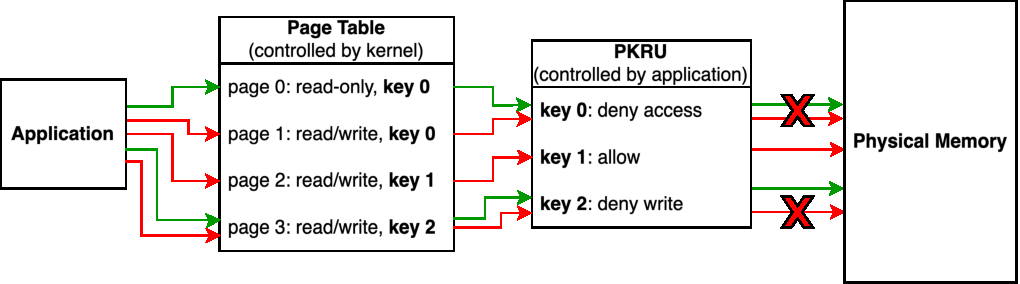
\includegraphics[width=\textwidth]{fig/mpk}
    \caption[Diagram of Memory Protection Keys]{Diagram of Memory Protection Keys. The kernel tags
    page table entries with a key (configurable with the \cc{pkey_mprotect} syscall). The user
    process can then restrict access to groups of pages by changing the permissions bits
    corresponding to a key in the PKRU register.}
    \label{f:mpk}
\end{figure}

This scheme allows a user program to manage its own sandbox: it can restrict or unrestrict regions
of memory at any time with a single register write -- without requiring expensive system calls,
context switches, or TLB flushes. It can't defend against all possible attacks: an attacker who can
take over the program's control flow may be able to use techniques such as return-oriented
programming to execute a \cc{wrpkru} instruction in order to disable the sandboxing and corrupt
protected memory. However, for our purposes of interoperability between memory-safe and
memory-unsafe code, it provides a low-overhead way to isolate the two and an effective line of
defense against memory corruption.

\paragraph{Prior Research} Prior research involving sandboxing using Memory Protection Keys includes
libmpk \cite{park:libmpk}, ERIM~\cite{vahldiek-oberwagner:erim}, Hodor~\cite{hedayati:hodor},
Cerberus~\cite{voulimeneas:cerberus}, Enclosure~\cite{ghoshn:enclosure} and
PKRU-safe~\cite{kirth:pkru}. libmpk by Park et al.~\cite{park:libmpk} implements a general-purpose
API that applications can use to manage protection keys, including a protection key virtualization
mechanism that applications can use to overcome the hardware limit of 16 protection keys; however,
it requires application developers to manually manage the keys and permissions associated with each
page of memory and configure the PKRU register appropriately before calling potentially unsafe
functions. ERIM by Vahldiek-Oberwagner et al.~\cite{vahldiek-oberwagner:erim} and Hodor by Hedayati
et al.~\cite{hedayati:hodor} explore the idea of software fault isolation with MPK, demonstrating
how this sandboxing can be used to protect applications in practice and implementing binary writing
techniques to prevent attackers from using control-flow hijacking to execute a \cc{wrpkru}
instruction and defeat the sandbox. Cerberus by Voulimeneas et al.~\cite{voulimeneas:cerberus}
extends this work further to defend against the possibility of unsafe code executing
attacker-controlled syscalls.

\paragraph{Automated Sandboxing} Enclosure by Ghoshn et al.~\cite{ghoshn:enclosure} automates the
process of creating sandboxed programs by extending mainstream programming languages with syntax to
manage sandboxing. PKRU-safe~\cite{kirth:pkru} by Kirth et al. directly addresses the problem of
sandboxing memory-unsafe code in memory-safe languages, and they do so using compiler extensions and
runtime instrumentation to perform provenance analysis of the program to determine what data
memory-unsafe code should have access to. Our work addresses the same problem as Kirth et al. --
sandboxing memory-unsafe code within memory-safe programs -- but our approach is implemented using
Rust's type system and procedural macros rather than requiring compiler or programming language
extensions.

\section{Other types of sandboxing} Sandboxing techniques can also be used to protect resources
other than memory, including filesystem, process, and networking resources. Linux provides
interfaces such as chroot~\cite {gnu:chroot}, seccomp/BPF~\cite {kim:mbox}, and Landlock~\cite
{linux:landlock} that can be used for this purpose. While our work limits the ability of sandboxed
code to take over its host program via memory corruption, it does not prevent sandboxed code from
compromising the system by e.g. writing to files or spawning a shell process; our work must be
combined with system call sandboxing techniques to prevent these attack vectors.
